\documentclass{article}
\usepackage[margin=1in]{geometry}
\usepackage{amsmath,amsthm,amssymb}
\usepackage{bbm,enumerate,mathtools}
\usepackage{tikz,pgfplots}
\usepackage{chessboard}
\usepackage[hidelinks]{hyperref}
\usepackage{multicol} % Problem 35
\usepackage{xstring} % Difficulty command
\usetikzlibrary{shapes.geometric}

\newenvironment{question}{\begin{trivlist}\item[\textbf{Question.}]}{\end{trivlist}}
\newenvironment{note}{\begin{trivlist}\item[\textbf{Note.}]}{\end{trivlist}}
\newenvironment{references}{\begin{trivlist}\item[\textbf{References.}]}{\end{trivlist}}
\newenvironment{related}{\begin{trivlist}\item[\textbf{Related.}]\end{trivlist}\begin{enumerate}}{\end{enumerate}}

\newcommand\score[1]{
\pgfmathsetmacro\pgfxa{#1+1}
\tikzstyle{scorestars}=[
  star,
  star points=5,
  star point ratio=2.25,
  draw,
  inner sep=3pt,
  anchor=outer point 5
]
  \begin{tikzpicture}[baseline]
    \draw[opacity=0] (0,-0.5) rectangle (0,0.2); % Workaround for whitespace at the bottom.
    \foreach \i in {1,...,4} {
      \pgfmathparse{(\i<=#1?"yellow":"gray")}
      \edef\starcolor{\pgfmathresult}
      \draw (\i*4.5ex,0) node[name=star\i,scorestars,fill=\starcolor]  {};
    }
  \end{tikzpicture}
}

\newcommand{\difficulty}[1]{%
  \IfEqCase{#1}{%
      {1}{
        
\begin{tikzpicture}[scale=0.7, baseline=0.9mm]%
          \definecolor{slopegreen}{rgb}{0.0, 0.5, 0.0}%
          \fill[slopegreen] (0.5,0.5) circle (0.5);%
        \end{tikzpicture}%
      }%
      {2}{
        
\begin{tikzpicture}[scale=0.7, baseline=0.9mm]%
          \definecolor{slopeblue}{rgb}{0.0, 0.44, 1.00}
          \fill[slopeblue] (0,0) rectangle (1,1);%
        \end{tikzpicture}%
      }%
      {3}{
\begin{tikzpicture}[scale=0.7, baseline=0.9mm]\fill (0,0.5)--(0.5, 0)--(1,0.5)--(0.5,1)--cycle; \end{tikzpicture}}%
      {4}{
\begin{tikzpicture}[scale=0.7, baseline=0.9mm]\fill (0.25,0)--(0,0.5)--(0.25,1)--(0.5,0.5)--cycle; \fill (0.75,0)--(0.5,0.5)--(0.75,1)--(1,0.5)--cycle;\end{tikzpicture}}%
      % you can add more cases here as desired
  }[\PackageError{difficulty}{Undefined difficulty level: #1}{}]%
}%
\newcommand{\rating}[2]{\difficulty{#1}\\\score{#2}\\}


\begin{document}
\rating{2}{3}
A problem inspired by a Project Euler problem: suppose an $n$-robot takes steps that are $1/n$ of a circle, and turns right
or left after every step.
\begin{figure}[!h]
  \centering
  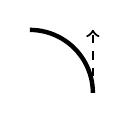
\begin{tikzpicture}[scale=0.8]
    \draw[thick, dashed, ->] (1,0)--(1,1);
    \draw[ultra thick, draw={}, domain=0:90] plot ({cos(\x) + 0}, {sin(\x) + 0});
  \end{tikzpicture}\\~\\~\\
  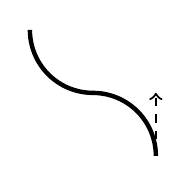
\begin{tikzpicture}[scale=0.8]
    \draw[thick, dashed, ->] (1,0)--(1,1);
    \draw[ultra thick, draw={}, domain=0:90] plot ({cos(\x) + 0}, {sin(\x) + 0});
    \draw[ultra thick, draw={}, domain=180:270] plot ({cos(\x) + 0}, {sin(\x) + 2});
  \end{tikzpicture}
  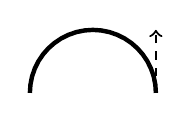
\begin{tikzpicture}[scale=0.8]
    \draw[thick, dashed, ->] (1,0)--(1,1);
    \draw[ultra thick, draw={}, domain=0:180] plot ({cos(\x) + 0}, {sin(\x) + 0});
  \end{tikzpicture}\\~\\~\\
  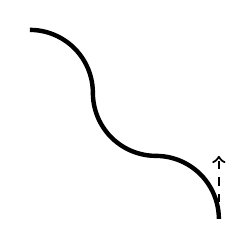
\begin{tikzpicture}[scale=0.8]
    \draw[thick, dashed, ->] (1,0)--(1,1);
    \draw[ultra thick, draw={}, domain=0:90] plot ({cos(\x) + 0}, {sin(\x) + 0});
    \draw[ultra thick, draw={}, domain=180:270] plot ({cos(\x) + 0}, {sin(\x) + 2});
    \draw[ultra thick, draw={}, domain=0:90] plot ({cos(\x) - 2}, {sin(\x) + 2});
  \end{tikzpicture}
  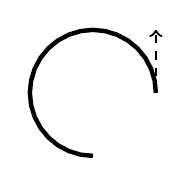
\begin{tikzpicture}[scale=0.8]
    \draw[thick, dashed, ->] (1,0)--(1,1);
    \draw[ultra thick, draw={}, domain=0:270] plot ({cos(\x) + 0}, {sin(\x) + 0});
  \end{tikzpicture}
  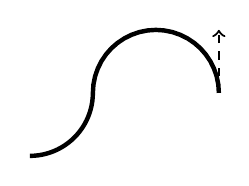
\begin{tikzpicture}[scale=0.8]
    \draw[thick, dashed, ->] (1,0)--(1,1);
    \draw[ultra thick, draw={}, domain=0:180] plot ({cos(\x) + 0}, {sin(\x) + 0});
    \draw[ultra thick, draw={}, domain=270:360] plot ({cos(\x) - 2}, {sin(\x) + 0});
  \end{tikzpicture}\\~\\~\\
  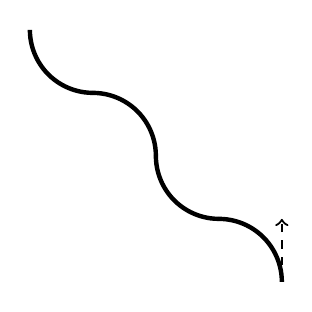
\begin{tikzpicture}[scale=0.8]
    \draw[thick, dashed, ->] (1,0)--(1,1);
    \draw[ultra thick, draw={}, domain=0:90] plot ({cos(\x) + 0}, {sin(\x) + 0});
    \draw[ultra thick, draw={}, domain=180:270] plot ({cos(\x) + 0}, {sin(\x) + 2});
    \draw[ultra thick, draw={}, domain=0:90] plot ({cos(\x) - 2}, {sin(\x) + 2});
    \draw[ultra thick, draw={}, domain=180:270] plot ({cos(\x)- 2}, {sin(\x) + 4});
  \end{tikzpicture}
  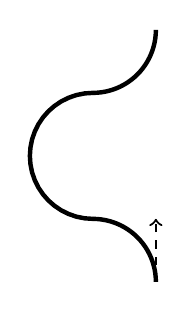
\begin{tikzpicture}[scale=0.8]
    \draw[thick, dashed, ->] (1,0)--(1,1);
    \draw[ultra thick, draw={}, domain=0:90] plot ({cos(\x) + 0}, {sin(\x) + 0});
    \draw[ultra thick, draw={}, domain=90:270] plot ({cos(\x) + 0}, {sin(\x) + 2});
    \draw[ultra thick, draw={}, domain=270:360] plot ({cos(\x) + 0}, {sin(\x) + 4});
  \end{tikzpicture}
  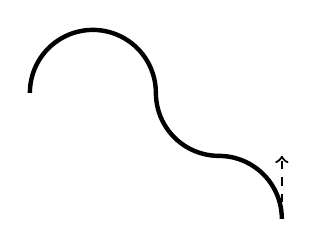
\begin{tikzpicture}[scale=0.8]
    \draw[thick, dashed, ->] (1,0)--(1,1);
    \draw[ultra thick, draw={}, domain=0:90] plot ({cos(\x) + 0}, {sin(\x) + 0});
    \draw[ultra thick, draw={}, domain=180:270] plot ({cos(\x) + 0}, {sin(\x) + 2});
    \draw[ultra thick, draw={}, domain=0:90] plot ({cos(\x) - 2}, {sin(\x) + 2});
    \draw[ultra thick, draw={}, domain=90:180] plot ({cos(\x)- 2}, {sin(\x) + 2});
  \end{tikzpicture}
  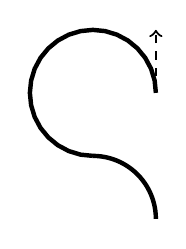
\begin{tikzpicture}[scale=0.8]
    \draw[thick, dashed, ->] (1,0)--(1,1);
    \draw[ultra thick, draw={}, domain=0:270] plot ({cos(\x) + 0}, {sin(\x) + 0});
    \draw[ultra thick, draw={}, domain=0:90] plot ({cos(\x) + 0}, {sin(\x) - 2});
  \end{tikzpicture}
  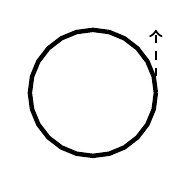
\begin{tikzpicture}[scale=0.8]
    \draw[thick, dashed, ->] (1,0)--(1,1);
    \draw[ultra thick, draw={}, domain=0:360] plot ({cos(\x) + 0}, {sin(\x) + 0});
  \end{tikzpicture}
  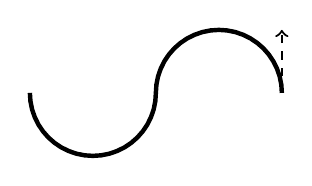
\begin{tikzpicture}[scale=0.8]
    \draw[thick, dashed, ->] (1,0)--(1,1);
    \draw[ultra thick, draw={}, domain=0:180] plot ({cos(\x) + 0}, {sin(\x) + 0});
    \draw[ultra thick, draw={}, domain=180:360] plot ({cos(\x) - 2}, {sin(\x) + 0});
  \end{tikzpicture}
  \caption{
    An example of distinct paths of $k$ steps (up to dihedral action) for a $4$-robot.
    $a(1) = 1$, $a(2) = 2$, $a(3) = 3$, and $a(4) = 6$.
  }
\end{figure}
\begin{question}
  \item How many walks exist such that the robot ends up at the original
    position and orientation after $k$ steps?
\end{question}
\begin{related}
  \item How many distinct paths exist for an $n$-robot, where the robot never
    retraces its steps?
  \item What if the robot is allowed to retrace its steps?
  \item What is the smallest radius that can contain a $k$-step walk if the robot
    cannot retrace its steps?
    (The robot returns to where it started in the same direction that it
    started.)
  \item Can smooth loop paths occur when the number of steps is not a multiple
    of $n$?
  \item What if the orientation of the path matters (i.e. \textit{not} counted
    up to dihedral action)?
  \item What if this is done on a torus, cylinder, or M\"obius strip?
  \item What if the robot cannot cross its own path?
\end{related}
\begin{references}
  \item \url{https://projecteuler.net/index.php?section=problems&id=208}
\end{references}

\end{document}
